\chapter {Model builder and Subcircuit builder}
\section {Model builder}


Spice based simulators include a feature which allow accurate modelling of semiconductor devices such as diodes, transistors etc. OSCAD Model Builder provides a facility to define a new model for devices such as diodes, MOS, BJT, JFET, IGBT, Magnetic core etc. Model Builder in OSCAD asks for a value of parameters depending on the type of the device for which a model is required. The parameter values can be obtained from a datasheet of the device. A newly created model can be exported to the model library and whenever required one can import it for different projects. Model Builder also provides a facility to edit existing models. 

Now let us take an example of Bridge rectifier circuit containing diode model 1N4007 and see how Model Builder works in Oscad.

In figure \ref{diode} you can see the diode model 1N4007 in the Bridge rectifier circuit.

\begin{figure}[h]%h stands for 'here'. If h is removed then the fig will go to the bottom or to the next page.
\begin{center}
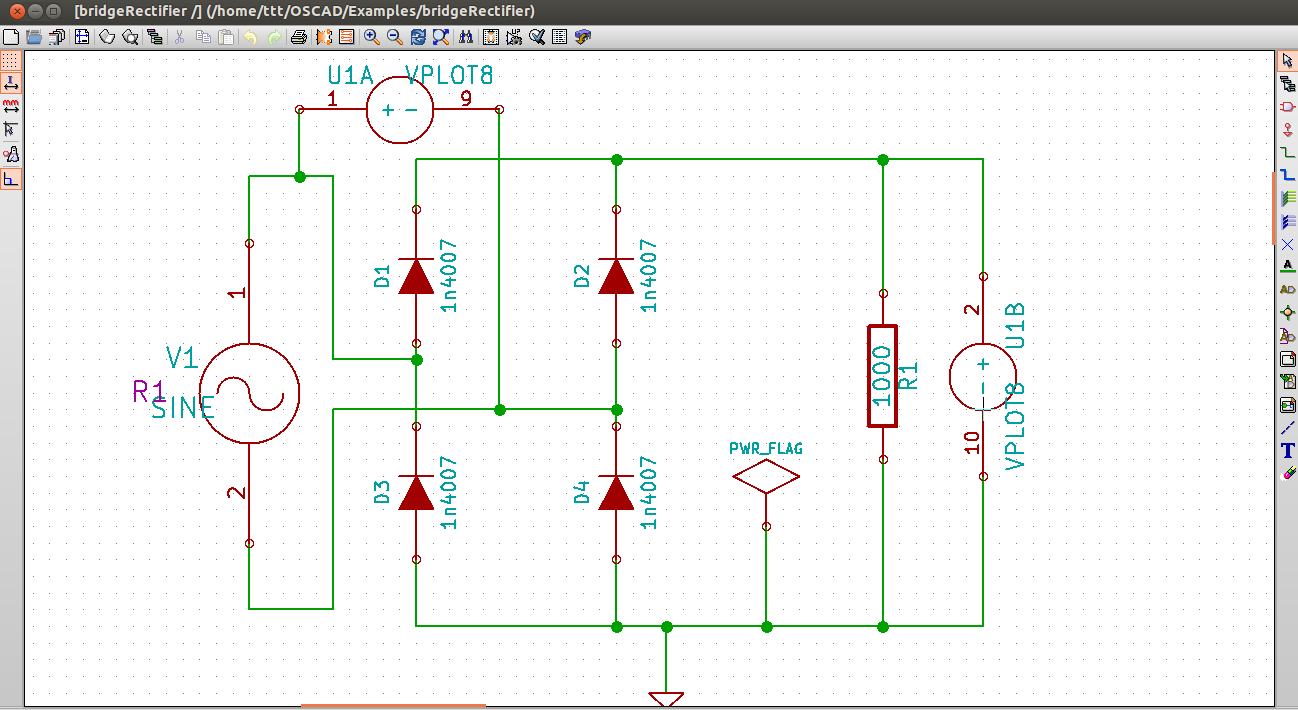
\includegraphics[width=1\linewidth]{figures/B-Rectifier-schematic.png}%If the fig is appearing too big/small, change the scaling factor 0.2
\caption{Diode model in bridge rectifier circuit}
\label{diode}
\end{center}
\end{figure}

Now to build a new model for the diode 1N4007 you will click on the Model builder of the toolbar of Oscad which will opens up the window shown in Figure \ref{edit} where it asks for the value of parameters for diode 1N4008. In this window you can change the values of the parameters for 1N4007 diode model as it is given in the datasheet and then save it.

\begin{figure}[h]%h stands for 'here'. If h is removed then the fig will go to the bottom or to the next page.
\begin{center}
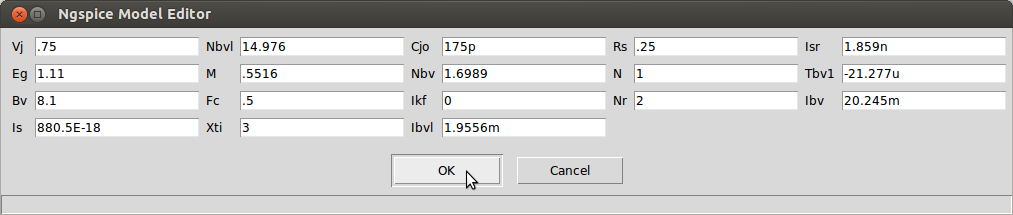
\includegraphics[width=1\linewidth]{figures/model-parameters.png}%If the fig is appearing too big/small, change the scaling factor 0.2
\caption{Edit model paramters}
\label{edit}
\end{center}
\end{figure}

Once a new diode model of 1n4007 is created it can be exported to the model library and whenever required one can import it for different projects which shown in the Figure \ref{export}.

\begin{figure}[h]%h stands for 'here'. If h is removed then the fig will go to the bottom or to the next page.
\begin{center}
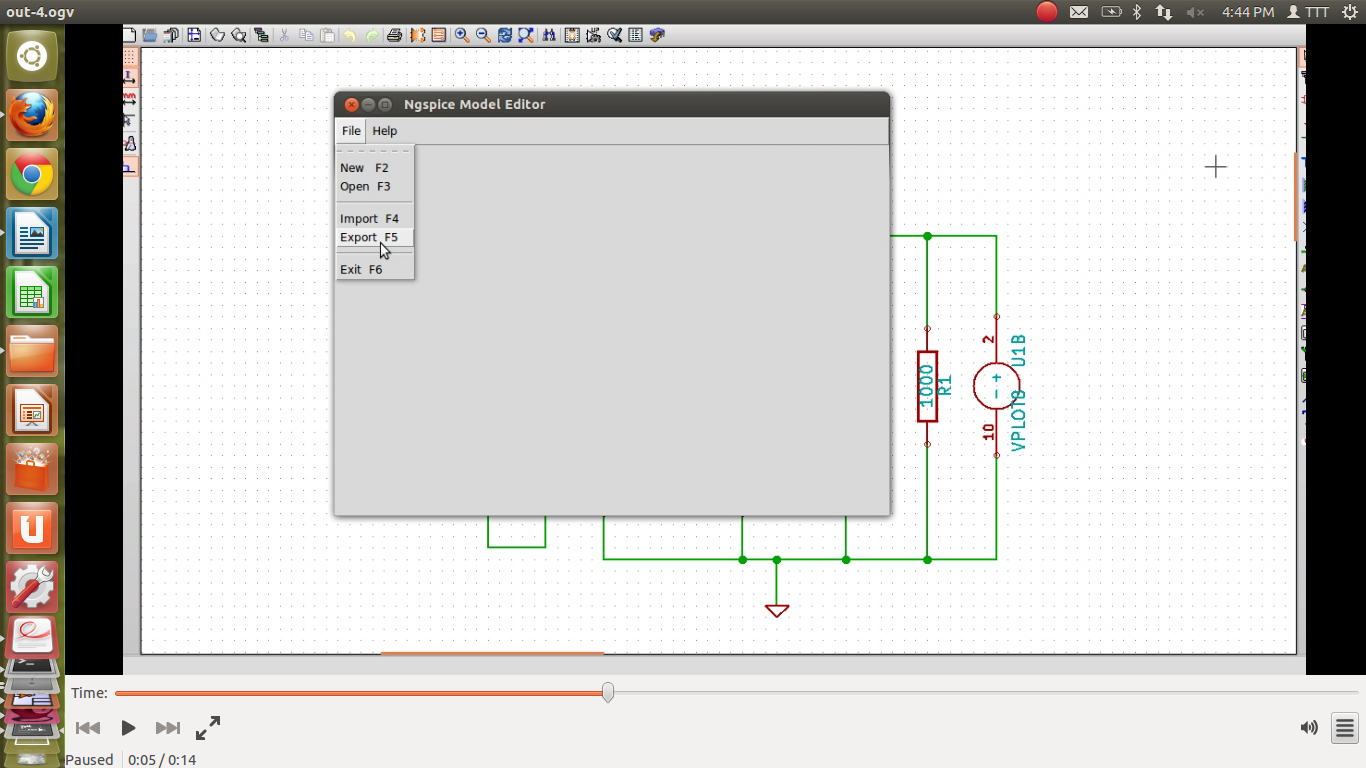
\includegraphics[width=1\linewidth]{figures/model-build-export.png}%If the fig is appearing too big/small, change the scaling factor 0.2
\caption{Export model}
\label{export}
\end{center}
\end{figure}




\section {Sub-circuit Builder:}
Sub-circuit is the way to implement hierarchical modeling. Once a sub-circuit for a component is created, user can use it for different circuits.

Oscad provides an easy way to create a sub-circuit in steps: 


\begin{figure}[h]%h stands for 'here'. If h is removed then the fig will go to the bottom or to the next page.
\begin{center}
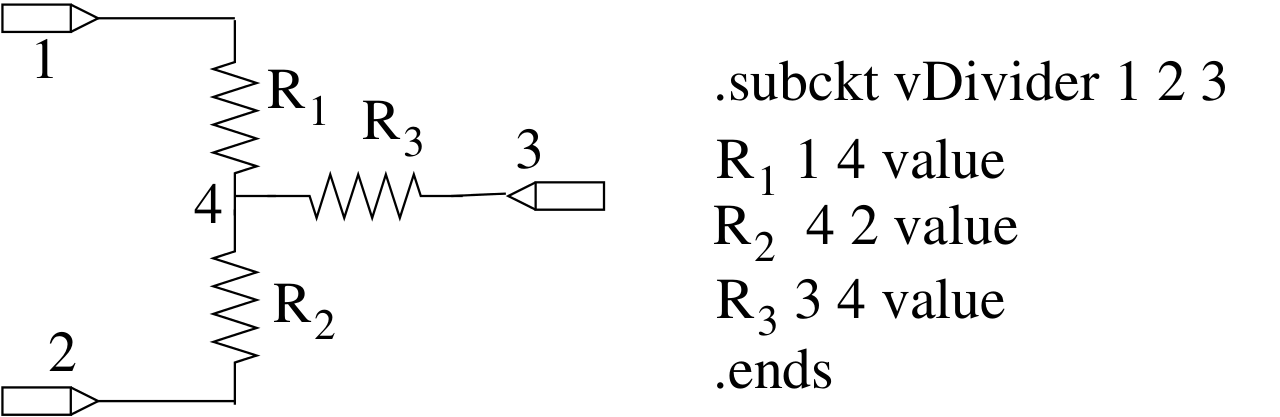
\includegraphics[width=1\linewidth]{figures/voltage-divider.png}%If the fig is appearing too big/small, change the scaling factor 0.2
\caption{Voltage divider subcircuit and definition}
\label{vsub}
\end{center}
\end{figure}

Firstly open Oscad sub-circuit builder. It will open the schematic editor (Eeschema).  Draw a sub-circuit. Then connect external pin of the sub-circuit to the component called “port” (provided by Oscad). Last step is to save it. 

Once saved, Sub-circuit builder finds out the pin connected to “port” and creates “.Subckt” line. In this line, the name of the component and the circuit nodes that connect sub-circuit to the main circuit are specified. The Ngspice compatible netlist is generated using the Netlist Converter 
explained in this section. The last line “.ends” is inserted in the sub-circuit definition. Now, the definition will be available for the project in which it is created. 

Figure \ref{vsub} shows a sub-circuit for voltage divider where nodes 1, 2 and 3 are external nodes and 4 is an internal node. The sub-circuit definition is given in the same figure. Once sub-circuit is created, it can be exported to the sub-circuit library and whenever required one can import it for different projects. The Oscad sub-circuit library already has some sub-circuit definitions for complex components such IC555, OpAmp 741 etc. The Oscad provides a library with 41 basic building blocks such as multiplier, limiter, basic gates, flip-flops, latches, D to A converter etc. Using these blocks, one can realize the most of the electronic circuits. 

Now let us take an example of building a subcircuit of IC 555 timer which is a part of Astable Multiovibrator circuit and see how Subcircuit Builder works in Oscad.

Once you click on the Subcircuit Builder of the Oscad it asks you to choose the subcircuit you wanted to create out of the list of all subcircuits present in the given circuit. It is shown in Figure \ref{msel}.


\begin{figure}[h]%h stands for 'here'. If h is removed then the fig will go to the bottom or to the next page.
\begin{center}
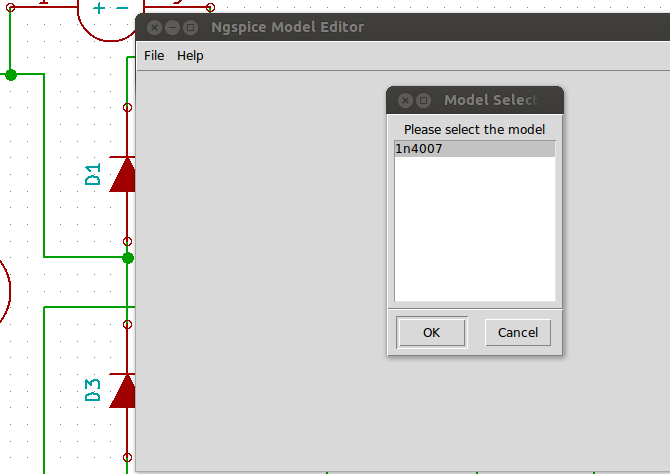
\includegraphics[width=1\linewidth]{figures/select-model.png}%If the fig is appearing too big/small, change the scaling factor 0.2
\caption{Select Model}
\label{msel}
\end{center}
\end{figure}


Once you select the subcircuit it opens up the Schematic Editor where you can create the subcircuit of IC 555 timer shown in Figure \ref{555}.

\begin{figure}[h]%h stands for 'here'. If h is removed then the fig will go to the bottom or to the next page.
\begin{center}
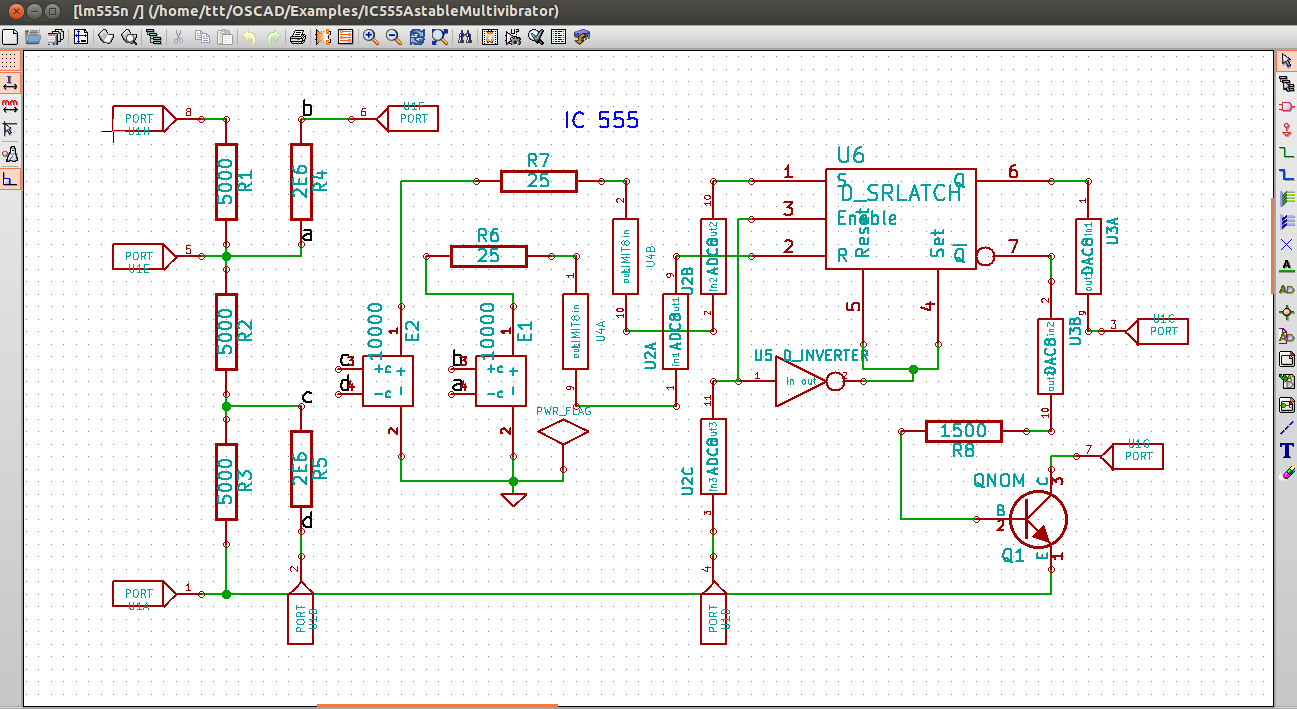
\includegraphics[width=1\linewidth]{figures/subcircuit.png}%If the fig is appearing too big/small, change the scaling factor 0.2
\caption{IC 555 timer subcircuit}
\label{555}
\end{center}
\end{figure}

Once you completed the creation of the subcircuit save it in respective project folder and close the Schematic editor. While you close the Shematic Editor a terminal pop-up of “Kicad to Ngspice netlist converter” will ask you to enter the value for the different parameters of subcircuit as shown in the Figure \ref{para}.

\begin{figure}[h]%h stands for 'here'. If h is removed then the fig will go to the bottom or to the next page.
\begin{center}
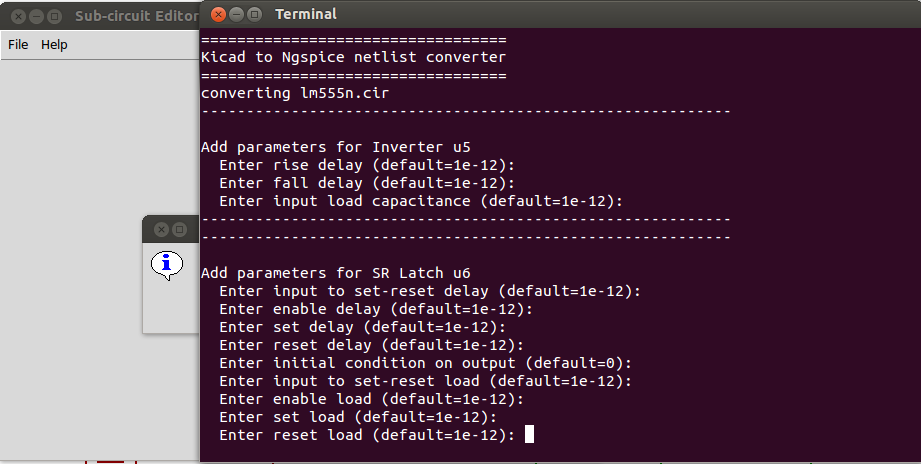
\includegraphics[width=1\linewidth]{figures/subcircuit-parameters.png}%If the fig is appearing too big/small, change the scaling factor 0.2
\caption{IC 555 timer subcircuit - parameters}
\label{para}
\end{center}
\end{figure}

At the end of the terminal you see that it tells you 
“The ngspice netlist has been written in lm555n.cir.out 
The scilab netlist has been written in lm555n.cir.ckt 
Press Enter to quit ” which says that netlist for the subcircuit is created. It is shown in the Figure \ref{net}.

\begin{figure}[h]%h stands for 'here'. If h is removed then the fig will go to the bottom or to the next page.
\begin{center}
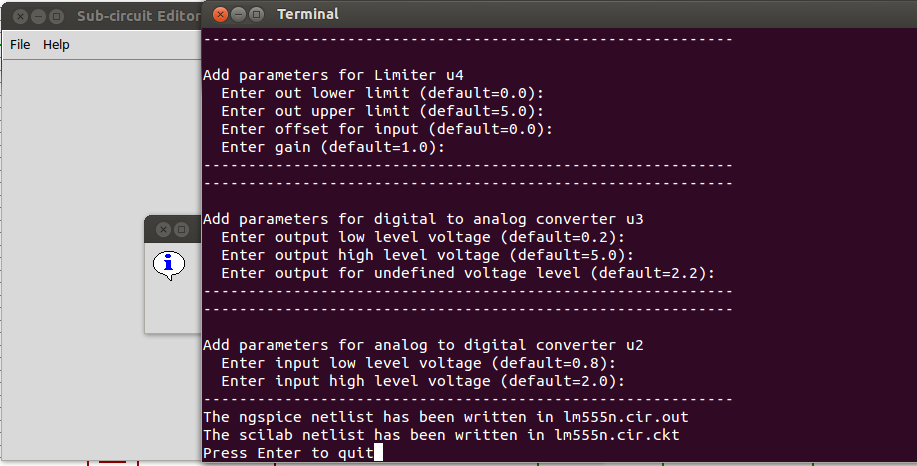
\includegraphics[width=1\linewidth]{figures/netlist-generation.png}%If the fig is appearing too big/small, change the scaling factor 0.2
\caption{Netlist conversion}
\label{net}
\end{center}
\end{figure}

Finally it says that “Created sub-circuit lm555n.sub”  as shown in Figure \ref{done} and then press ok to complete the subcircuit creation. 

\begin{figure}[h]%h stands for 'here'. If h is removed then the fig will go to the bottom or to the next page.
\begin{center}
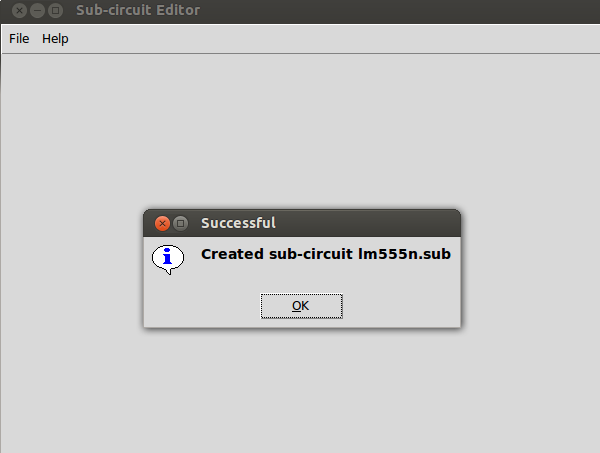
\includegraphics[width=1\linewidth]{figures/subcircuit-created.png}%If the fig is appearing too big/small, change the scaling factor 0.2
\caption{Subcircuit creation successfull}
\label{done}
\end{center}
\end{figure}

Once sub-circuit is created, it can be exported to the sub-circuit library as shown in Figure \ref{exp} and whenever required one can import it for different projects.

\begin{figure}[h]%h stands for 'here'. If h is removed then the fig will go to the bottom or to the next page.
\begin{center}
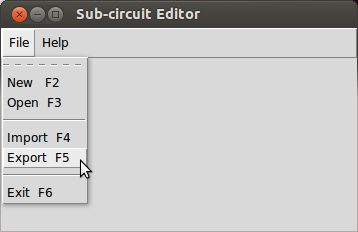
\includegraphics[width=1\linewidth]{figures/export-subcircuit.png}%If the fig is appearing too big/small, change the scaling factor 0.2
\caption{Export Subcircuit}
\label{exp}
\end{center}
\end{figure}

Finally close the subcircuit editor window.









